\chapter{引言}
\label{cha:intro}

\section{选题背景}
\label{sec:background}

随着时代的发展,人们对于数字娱乐媒体形式的需求愈发从文字、图片转向视频,这一点一方面得益于
网络传输技术的发展所带来的更大的带宽,另一方面,视频编码技术的进步,使得同样质量的视频所需要
的数据量变小,视频体积的减小方便了其传播与分享。

自20世纪80年代起,人们开始注重对数字视、音频的压缩与存储,著名的MPEG正是于这一时期成立,并先后
为视频编码制定了H.261、H.263等一系列标准,并于2003年与ITU-T的视频编码专家组VCEG合作,正式发布
了影响深远的H.264视频编码标准。然而,在人们对视频分辨率追求愈发提高的今天,1080p甚至4k等高分辨
的视频已大幅超出了H.264的能力,且对于60fps的高帧率以及更高压缩率等要求,也无法被纳入H.264的框架
内,H.265应运而生。H.265作为新一代的视频编码标准,力求在更高的分辨率、帧率、压缩率等方面成为H.264
的上位替代。

尽管MPEG组织所定制的一系列视频编码标准取得了良好的效果,但其高昂的使用许可费用使得无数开发研究者
望而却步。为此,Google于2010年启动了WebM项目,该项目旨在制定高效且不需要版权费的视频编码标准。
作为项目的一部分,2010年,视频编码标准VP8出炉,并成功应用于Hangouts;而2013年,新一代的VP9定制
完成,并在应用于Youtube,相较于H.264,其减少了30\%-40\%的带宽,且这些带宽上的收益都来自于软件
解码。

\begin{figure}[H] % use float package if you want it here
  \centering
  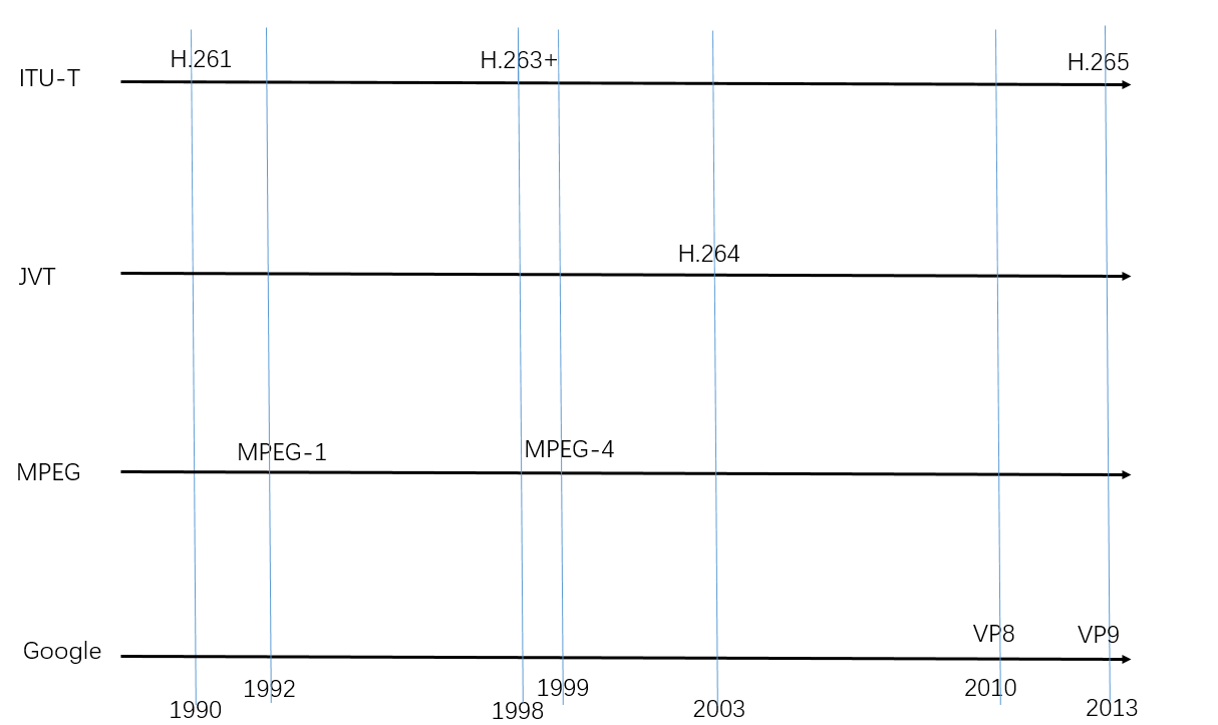
\includegraphics[width = 0.8\textwidth]{intro-coding-timeline}
  \caption{视频编码标准发展}
\end{figure}

本着开源、免版权税的原则,2015年,开源媒体联盟AOM成立,并为定制VP9的接班者、下一代的开源免版权
视频编码标准——AV1而努力。近年来直播行业的兴起,使得直播系统成为互联网带宽的主要消耗者,因此AV1
应在VP9的基础上进一步减少编码视频所用的比特数,且直播的特点决定了降低解码端复杂度应是新标准的目标
之一。历经3年的开发时间,2017年底AV1的代码框架初步完成,初版的编码器效率极低,耗时极长,对编码
器的优化亟待进行。

AV1虽为新生的视频编码标准,但其主体框架H.264、H.265、VP9等大同小异。如前所述,AV1代码框架近期初步
搭建完成,其优化空间是广阔的,又因为其在框架结构上与之前的标准大同小异,因此许多针对H.264、H.265、VP9等
视频编码标准的优化算法,是极有可能移植到AV1上并展现出良好效果的。

\section{研究内容}
\label{sec:content}

本文主要针对新的视频编码标准AV1做优化,在以视频质量几乎不变或是有轻微降低的前提下,尽量提升视频
编码的速度。

考虑到AV1编码标准是一个新标准,其代码框架尚处于比较初步的阶段,几乎没有做过优化,因此,优化算法
主要考虑将已有的、成功应用于过去的编码标准的优化算法移植过来。视频编码流程较为复杂,整个流程中有
数点可以进行针对性的优化:例如在将视频帧划分为块时,既可以对划分算法本身进行优化,也可以通过预测,
尽可能早地终止划分过程,从而达到加速的目的;在运动估计方面,针对运动估计过程或是与运动矢量进行优化
的算法也有许多;在预测方面,帧间预测和帧内预测两大预测模式,不同的预测算法也可能带来极大的加速。

在算法上,本文针对视频帧划分为块的这一过程进行优化。这一过程中,帧被不断划分为更小的矩形,并
以树结构进行存储,对于每个树节点,如何划分为子树是一个复杂且耗时的过程。若能提前判断某一节点不需要
再进行划分,则该节点的子树的计算均可被省略,由此大大提升计算效率,加速编码过程。这种通过更早地终止编码树
分叉、从而实现视频编码的加速的思想,就是本文所研究的加速算法的核心。

\section{研究现状}
\label{sec:current-status}


对于尚处于开发中的AV1标准,笔者没有找到较好的针对帧划分为块这一过程,以早终止为思路进行优化的相关工作。
因此,笔者把目光放在H.264与H.265这两个被人研究较多的编码标准,通过考察这两种标准上的早终止优化算法
现状,来进行AV1编码标准下的移植。

\begin{table}[htb]
  \centering
  \begin{minipage}[t]{0.8\linewidth}
    \caption{H.264、H.265、AV1比较}
    \begin{tabularx}{\linewidth}{lXXX}
      \toprule[1.5pt]
       & {\heiti H.264} & {\heiti H.265} & {\heiti AV1} \\\midrule[1pt]
      宏块大小 & 16 x 16 & 64 x 64 & 128 x 128 \\
      四叉编码树 & 否 & 是 & 是 \\
      划分种类 & 7 & 4 & 10 \\
      \bottomrule[1.5pt]
    \end{tabularx}
  \end{minipage}
\end{table}

H.264标准中编码树的概念比较薄弱,对于某一视频帧,首先会被划分为宏块,而每一宏块有且仅有七种划分模式,
在这七种模式中选择最优的一种即是优化的关键。可能的算法包括:根据块的运动矢量MV做一些统计上的分析并与阈值比较,从而提前终止
运动估计过程 \cite{xu2003efficient} ;或者是 Libo Yang和Keman Yu等人(2005)\cite{yang2005effective}
提出的根据宏块对应的运动矢量预测宏块的划分模式的方法等。由于H.264没有采用四叉编码树的结构,因此对其
进行的优化工作在移植上有一定难度,但仍具有一定参考价值。

%介绍H.265部分
H.265则与AV1更为相近,同样是采用四叉编码树进行组织,因此对H.265标准进行的优化工作在移植时相对容易。
真对H.265的早终止优化,一种思路是Shen Xiaolin 等人使用SVM进行分类预测\cite{shen2013cu}。该方法
效果较好但缺点在于他们的工作中,对于SVM中特征空间的选取十分复杂,由此在移植时将带来极大的不确定性。
也有一些相对清晰且易于移植的方法,例如:Jongho Kim等人提出了基于先前跳过的CU的率失真代价进行预测,
从而提前终止CU划分的方法 \cite{kim2012adaptive};类似的,K Choi和SH Park等人也使用率失真代价作为
衡量标准,提出了对编码树进行剪枝的算法 \cite{choi2011coding}。可以看到,使用率失真代价进行比较,从而
提前终止CU的划分,是一种有效且易于移植的方法。

\section{论文结构}

本文章节安排如下:

\textbf{第 \ref{cha:coding} 章} \; 以VP9为例介绍视频编码流程,在此基础上介绍AV1

\textbf{第 \ref{cha:algorithm} 章} \; 介绍本项目最使用的早终止算法 

\textbf{第 \ref{cha:result} 章} \; 展示实验流程及结果,并加以分析

\textbf{第 \ref{cha:conclusion} 章} \; 总结本项目所做的工作,并对未来可能进行的改进加以展望